The tool used in this work to achieve single-atom control is optical tweezers: by focusing a laser beam to a small enough spot it has been shown that under the right conditions, this trap can house at most one atom (\cref{sec:LoadingAtoms}).
Subsequently, \cref{sec:DiffractionLimit} introduces the fundamental limit on the tweezer geometry. 
In \cref{sec:TweezersPractice} practical constraints of the specific setup used are introduced, after which \cref{sec:MeasuringTweezer} introduces the optical setup used to measure the optical dipole presented in \cref{sec:TweezerRadial,sec:Tweezer3D}.

\section{Loading Single Atoms}\label{sec:LoadingAtoms}

Single atom loading was first demonstrated by \cite{Schlosser2001}.
In \cite{Schlosser2002} it is described by an elegant model taking into account one-body as well as two-body loss terms. 
Denoting the average number of atoms in the dipole trap by $N$, we can write for the time evolution of $N$ \cite{Schlosser2002} 

\begin{equation}\label{LoadingTweezer}
	\frac{\text{d}N}{\text{d}t} = \alpha - \gamma N - \beta N(N-1),
\end{equation}
where the first term $\alpha$ is the loading rate or the amount of atoms entering the trap.
Next, $\gamma$ is the atom loss as a result of collisions with the background gas, so this is effectively a one-body loss term.
Lastly, $\gamma$ is a measure for the mainly two-body loss as a result of light-assisted collisions.
In this model, 3-body terms and higher are omitted.
In the regime $\beta \gg \gamma$, two-body loss rates are dominant over one-body contributions. 
We can now look at two distinct scenarios of an additional atom entering the trap:

\begin{itemize}
	\item Starting from 0 atoms present in the tweezer: an additional atom entering will now load the trap to $N=1$. 
	
	\item Starting from $N=1$: when an additional atom is loaded, the atoms will immediately kick out each other because of the tiny tweezer volume and strong light intensity from the MOT beams leading to $N=0$.
	
	\item In the situation that $N>1$, the atoms will be kicked out of the trap in pairs as a result of light-assisted collisions, until either $N=0$ or $N=1$.
\end{itemize}
Apparently, a loading event can lead to either 0 or 1 atom in the tweezer, both with $\sim 50\%$ probability. 
This is known as the collisional blockade mechanism and is also known as parity projection.
Experimentally demonstrated by \cite{Schlosser2001} and \cite{Schlosser2002} showed this effect to exits for 3 orders of magnitude in the loading rate $\alpha$.
Satisfying $\beta \gg \gamma$ can be done by keeping $\gamma$ to a minimum by going to the ultra high vacuum regime.
We intent to go to a pressure of the order of $10^{-10}$ mbar. In addition $\beta$ is maximized by going to high light-intensities and small trapping volumes. 
The remainder of this chapter is dedicated on how to minimize this trapping volume.

\section{Diffraction Limit}\label{sec:DiffractionLimit}

The smallest achievable spot size is governed by the diffraction limit; because of the wave character of light, there is a fundamental limit to the smallest spot size one can focus this wave, even in the absence of aberrations.
Diffraction theory is elegantly described by Fourier optics \cite{Goodman2005}. 
We present a short derivation of an important result from Fourier optics used throughout this work here, for the specific case of circular apertures.
For a more elaborate derivation, the reader is directed to \cref{Goodman2005}.

\begin{mdframed}
    \subsection*{Intermezzo Fourier Optics}
    
    When using a lens to form a focus, the lens will have a finite aperture.
    The light impinging on this aperture will show diffraction as a result.
    We call its complex amplitude $E(x',y')$ and position the aperture at axial coordinate $z = 0$ on the optical axis.
    After the aperture, the light field will show diffraction, described by the Fresnel diffraction integral in Cartesian coordinates \cite{Goodman2005}, leading to the complex field amplitude $E(x,y,z)$ after the aperture of 

    \begin{equation}\label{eq:FresnelDiffraction}
        E(x,y,z) = 
        \frac{e^{ikz}}{i \lambda z} \iint_{-\infty}^{\infty} E(x',y',0) \exp{\left(\frac{ik}{2z}\right)} \exp{\left[(x-x')^2+(y-y')^2\right]} dx'dy'.
    \end{equation}
    In \cref{eq:FresnelDiffraction}, $\lambdaup$ is the wavelength, $k=2\pi/\lambdaup$ the wavenumber. The aperture contribution is hidden in the term $E(x',y',0)$, which is zero when the condition $x'^2+y'^2>R^2$ is met, where $R$ is the radius of the circular aperture.
    During this work, we are usually not immediately interested in describing the light shortly after the aperture, but rather in the far field, motivating the use of the following Fraunhofer criterion
    
    \begin{equation}\label{eq:FraunhoferCriterion}
        z \gg \frac{k R^2}{2},
    \end{equation}
    While \cref{eq:FraunhoferCriterion} is in practice not met, it does near the focal point of a lens because a lens projects an image from infinity in its focal a length $f$ away. 
    Inserting \cref{eq:FraunhoferCriterion} in \cref{eq:FresnelDiffraction} yields the Fraunhofer diffraction integral:
    
    \begin{equation}\label{eq:FraunhoferDiffraction}
        E(x, y, z)=\frac{e^{i k z} e^{i k\left(x^{2}+y^{2}\right)/2}}{i \lambda z} \iint_{-\infty}^{\infty} E(x', y',0) \exp \left[\frac{-ik}{z}(x x'+y y')\right] dx' dy'.
    \end{equation}
    Because in this work we will usually compute the intensity as the absolute value squared, which will drop the phase factor in front of \cref{eq:FraunhoferRTheta}. Again, we only have to integrate over contributions within the aperture radius, such that we can write 
    
    \begin{equation}\label{eq:FraunhoferSimplified}
        E(x,y,z) \propto 
        \iint_{\text{aperture}} E(x',y') \exp{\left[- \frac{ik}{z}(xx'+yy')\right]}dx'dy'.
    \end{equation}
    This is the 2D spatial Fourier transform (in $x$ and $y$), with respectively spatial frequencies $f_x = x/\lambdaup z$ and $f_y = y/\lambdaup z$ and will be frequently used in this work.
\end{mdframed}

\noindent For circular apertures, a description in cylindrical coordinates is more natural. 
Using the standard definitions for cylindrical coordinates, \cref{eq:FraunhoferSimplified} can be written as

\begin{equation}\label{eq:FraunhoferRTheta}
    E(r,\theta, z) \propto \iint_{\text{aperture}} E(r') \exp{\left[
    -\frac{i k r r'}{z} \cos{(\theta-\theta')} 
    \right]}r'dr'd\theta'.
\end{equation}
Using the integral definition of the Bessel function of the first kind\footnote{$J_0(x) = \frac{1}{2\pi} \int_0^{2\pi} \exp{(i x \cos{\alpha})} d\alpha$}, this simplifies to
\begin{equation}\label{eq:FourierBessel}
    E(r,z) \propto 2\pi \int_0^{\infty} E(r') J_0\left( \frac{k r r'}{z}\right) r'dr',
\end{equation}
which is the Fourier-Bessel or Hankel transform.
Initially, we limit ourselves to potentials in the focus of the lens only, such that $z=f$. Also, for optical tweezers applications a fair assumption is that the incident light field is a Gaussian beam, with 'input' waist $w_i$, such that the light field is up to a normalization constant $A$

\begin{equation}\label{eq:GaussianAperture}
    E(r')=
    \begin{cases}
        A e^{- r'^2/w_i^2},& \text{if } r' < R\\
        0,               & \text{otherwise}.
    \end{cases}
\end{equation}
Substituting \cref{eq:GaussianAperture} in \cref{eq:FourierBessel} yields

\begin{equation}\label{eq:FourierBesselAperture}
    E(r) \propto \int_0^R e^{-r'^2/w_i^2} J_0\left(\frac{k r r'}{f}\right)r'dr'.
\end{equation}
\Cref{eq:FourierBesselAperture} is analytically solvable for specific cases \cite{Madjarov2020}.
Letting $w_i/R$ go to infinity, which is to treat the incident Gaussian beam as a plane wave, we can neglect the exponential term in \cref{eq:FourierBesselAperture}. 
The integral is now tractable, yielding for the field amplitude

\begin{equation}\label{eq:AiryField}
    E(r) \propto \frac{f}{kRr} J_1\left(\frac{k R r}{f}\right).
\end{equation}
Taking the absolute value squared and normalizing yields for the intensity the Airy function:

\begin{equation}\label{eq:NormalizedPSF}
    \frac{I}{I_0} = \left[
    \frac{2J_1(k r R/f)}{k r R/f}
    \right]^2.
\end{equation}
Which is plotted in \cref{fig:AiryPlots}, as well as the circle that results from \cref{eq:NormalizedPSF} known as the Airy disk.
Including the axial variable $z$ again, the optical response of a perfect lens to this plane wave is known as the \ac{PSF}, which we will use in \cref{sec:Tweezer3D}.
Solving for the first zero of \cref{eq:NormalizedPSF}, and introducing the definition of \ac{NA}: $\text{NA} = n \sin{\theta} =  R/f$, where $\theta$ is the maximum half angle and $n\approx1$ in air, yields for the radius of this Airy disk:

\begin{figure}
    \centering
    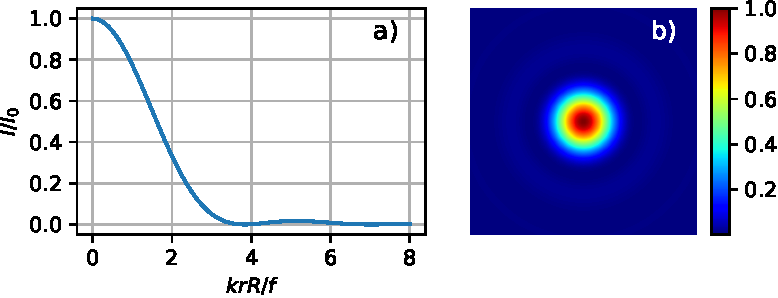
\includegraphics[width = 0.9\linewidth]{figures/AiryDisk.pdf}
    \caption{Normalized plots of the Airy function for \textbf{a)} only the radial coordinate (normalized in units of $f/kR$) as well as \textbf{b)} a 2D plot: the Airy disk.}
    \label{fig:AiryPlots}
\end{figure}

\begin{equation}\label{eq:Abbe}
    d_1 = 0.61 \frac{\lambdaup}{\text{NA}}.
\end{equation}
This result is known as the Abbe limit or diffraction limit \cite{Abbe1882} and it is the smallest feature a lens can produce.
To minimize $d_1$ in \cref{eq:Abbe} we can thus increase the \ac{NA} of our imaging system. 
In this work we will use $\text{NA} = 0.5$\footnote{For high NA imaging systems however, the paraxial approximation which was used to simplify the diffraction integral is no longer a priori true. 
Though, \cite{Chon2007} present a derivation of \cref{eq:Abbe} using a different diffraction theory that does not require paraxial approximation and showed that for collimated laser beams \cref{eq:Abbe} has negligible error even for $\text{NA} = 1$. 
We will assume we can still apply \cref{eq:Abbe} for $\text{NA} = 0.5$.}

In practice, it is not convenient to use \cref{eq:FourierBesselAperture} to fit data and it is more convenient to use a simpler function. 
A Gaussian function is commonly used, and can sometimes even fit better than \cref{eq:FourierBesselAperture} because the rings of the Airy disk are easily deformed because of aberrations \cite{Knottnerus2018}. 

\mbox{}\par
\begin{mdframed}
    \subsection*{Intermezzo Gaussian Beams}\label{sec:GaussianBeams}
    
    Because we will frequently use the parameters of a Gaussian beam, we will review them here. 
    Starting from Maxwell equations, one can derive under paraxial approximation a description of the transverse electromagnetic mode (TEM\textsubscript{00}) \cite{Leeuwen2017} for the electric field $E$.
    This Gaussian beam is most conveniently written down in cylindrical coordinates $\{r,z\}$:
    
    \begin{equation}\label{eq:GaussianBeam}
    	E(r,z) = \frac{w_0}{w(z)} \exp{\left(\frac{-r^2}{w^2(z)}\right)} \exp{\left[-ikz-i\frac{kr^2}{2R(z)} - i\psi(z)\right]},
    \end{equation}
    with parameters
    
    \begin{equation}\label{eq:GaussianBeamParameters}
    	k = \frac{2\pi}{\lambdaup}, \quad 
    	w(z) = \sqrt{w_0 + \frac{z^2}{z_R^2}}, \quad \text{and} \quad
    	R(z) = z \left(1 + \frac{z^2}{z_R^2}\right).
    \end{equation}
    Respectively, the wave number in terms of the wavelength $\lambdaup$, the beam waist, the radius where the field drops $1/e$ in terms of $w(z)\equiv w_0$ and $R(z)$ is the wavefront curvature. $z_R$ is the Rayleigh range, the distance along the optical axis where the beam waist has increased a factor of $\sqrt{2}$: $w(z=z_R) = \sqrt{2}w_0$.
    Finally $\psi(z)$ is an extra phase term originating from the curvature of the wavefront known as the Gouy phase.
    We find the intensity of the Gaussian beam by taking the absolute value squared:
    
    \begin{equation}\label{eq:GaussianBeamIntensity}
    	I(r,z) = I_0 \frac{w_0^2}{w^2(z)} \exp{\left(\frac{-2r^2}{w^2(z)}\right)}.
    \end{equation}
    A sketch of a Gaussian beam profile is given in \cref{fig:GaussianBeam}, showing the $1/e$ field radius, or $1/e^2$ intensity radius $w_0$ and the Rayleigh range $z_R$. 
    
    \vspace*{3mm}
    \centering
        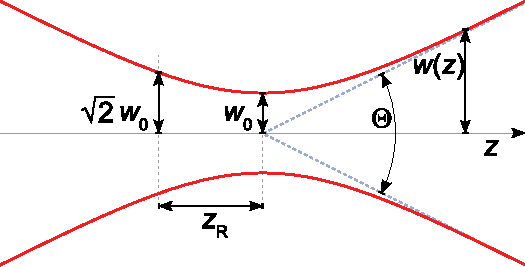
\includegraphics[width=0.5\linewidth]{figures/GaussianBeam.pdf}
        \captionsetup{margin=0mm}%somehow this works
        \captionof{figure}{Gaussian beam profile and some key parameters used in this work, the beam waist $w_0$ and Rayleigh range $z_R$. 
        Figure adapted from \cite{Hermans2009}.}
        \label{fig:GaussianBeam}
\end{mdframed}

Fitting this Gaussian as closely as possible to an Airy pattern using a least-squares optimization, it can be shown that the equivalent Gaussian waist is \cite{Zhang2007}.

\begin{equation}\label{eq:GaussianAiryFit}
    w = 0.42 \frac{\lambdaup}{\text{NA}}
\end{equation}
This the agreement of this approximation is excellent, but it is only valid near the center region of the Gaussian. 
If our measured waist is at this limit, the system is said to be diffraction limited, that is: the spot size is limited because of the wave character of light and not because of optical aberrations. 

At this point, it is instructive to get a feeling for the spatial profile of the dipole potential.
From \cref{eq:Stark} we know that the potential of the tweezer is proportional to the light intensity. 
Assuming the dipole potential can be described by a Gaussian, which is valid \cite{Zhang2007} near the center of the trap, the potential $U(r,z)$ in cylindrical coordinates is

\begin{equation}\label{eq:GaussianPotential}
    U(r,z)=\frac{-U_{0}}{1+z^{2} / z_{R}^{2}} \exp \left[\frac{-2 r^{2}}{w_{0}^{2}\left(1+z^{2} / z_{R}^{2}\right)}\right],
\end{equation}
where be used \cref{eq:GaussianBeam,eq:GaussianBeamParameters}.
\Cref{eq:GaussianPotential} is plotted in \cref{fig:GaussianPotential} as function of the normalized radial $r/w_0$ and axial $z/z_R$ coordinates. 
The figure is not to scale: the Rayleigh range $z_R$ is typically bigger than the waist $w_0$.
We will use equations of the form \cref{eq:GaussianPotential} to fit opical tweezer potentials.

\begin{figure}
    \centering
    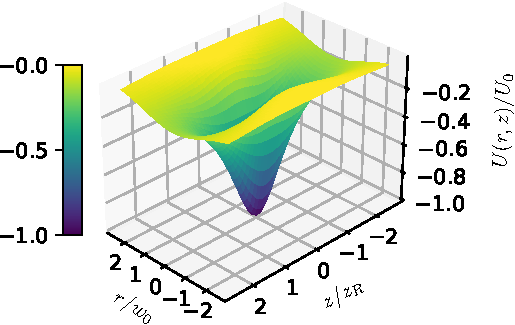
\includegraphics[width=.56\linewidth]{figures/GaussianPotential.pdf}
    \caption{Normalized potential $U/U_0$ for a Gaussian trap shape as a function of the normalized cylindrical coordinates $r/w_0$ and $z/z_R$. Not to scale: typically the Rayleigh range $z_R$ is larger than the beam waist $w_0$.}
    \label{fig:GaussianPotential}
\end{figure}



\section{The Microscope Objective}\label{sec:TweezersPractice}

To minimize \cref{eq:Abbe} and consequently minimize the volume of the optical trap, we need the highest possible numerical aperture, which are typically obtained by microscope objectives. 
But there are other demands on the microscope objective: the \ac{MOT} and subsequent \ac{ODT} are made in a vacuum chamber so the beam traverse a vacuum viewport, requiring:

\begin{enumerate}
    \item Ultra-long working distance (the distance between the trap and the lens). For a single lens, this is equivalent to the focal length $f$ of course, though for a compound microscope objective this does not have to be the case.
    
    \item Glass-thickness compensation. The relatively thick vacuum viewport will introduce a significant amount of aberrations for high NA and therefore large angles. It is possible to correct for this by having additional optics inside of the objective which will pre-correct for this error.
\end{enumerate}
To achieve this, we chose the G Plan Apo microscope objective from \textit{Mitutoyo}, as also used by \cite{Manuel2016,Ebadi2021}. 
This is an infinity-corrected objective, meaning light collected in its focused is imaged at infinity (parallel beam) and an additional field lens is used to focus this image, such that the magnification is 

\begin{equation}\label{eq:InfinityMagnification}
    M = \frac{
    f_{\text{FL}}
    }{
    f_{\text{obj}}
    }
\end{equation}
where $f_{\text{FL}}$ is the focal length of the field lens and $f_{\text{obj}}$ the equivalent focal length of the objective\footnote{For a compound microscope objective, equivalent focal length means the focal length the objective would have when replaced by a single lens.}.
This has the advantage that it is more flexible than a finite-conjugate corrected objective, as it allows to place additional optics between the laser and the objective without as well as optics between the objective and field lens without changing alignment.
Additionally, it allows flexible variation of the magnification according to \cref{eq:InfinityMagnification}.
Relevant specifications of the objective for applications in optical tweezers are shown in \cref{table:MitutoyoSpecs}. 
From compound objectives, the equivalent focal length $f_{\text{obj}}$ is defined in terms of the \ac{NA} and the back aperture radius of $R$ as $f_{\text{obj}} = R / \text{NA}$, meaning the back aperture radius is 2 mm.

\begin{table}[h]
    \centering
    \caption{Key specifications of the objective from manufacturer Mitutoyo.}
    \label{table:MitutoyoSpecs}
    \begin{tabular}{l | l}
        \textbf{Specification}       & \textbf{Value} \\ \hline 
        NA                           & 0.5            \\ \hline
        Glass thickness compensation\footnote{We assume 3.5 mm of N-BK7 glass is used here, which has a slightly different refractive index than quartz for example.} & 3.5 mm         \\ \hline
        Equivalent focal length      & 4 mm           \\ \hline
        Working distance             & 15.08 mm      
    \end{tabular}
\end{table}
\noindent Because this objective was designed for wavelengths in the visible range, it is probable that all of the lenses inside it are coated with a reflection coating that does not work well for the 800 nm regime. 
This is indeed the case, as we measured the transmission of the objective to be just $(47 \pm 3)\%$ at 820 nm. 
Significant loss of laser power is therefore unavoidable.
But this is not the only source of laser power loss: in producing the perfect \ac{PSF} we assumed plane wave illumination ($w_i \gg R$, but in reality this is impractical: assuming the beam is aligned with the center of the aperture, the fraction of optical power $P/P_0$ traversing the aperture as a function of the incident waist $w_i$ is

\begin{equation}\label{eq:fracPowerCircular}
    P/P_0 = 1 - e^{-2w_i^2/R^2},
\end{equation}
which tends to zero for very wide beams (plane waves), which is not practical. 
On the other hand, the other extreme case is $w_i \ll R$: the waist is much smaller than the aperture and according to \cref{eq:fracPowerCircular} all of the power is transmitted through the aperture.
We can have a look at the shape of the resulting light potential: letting the integration boundary of \cref{eq:FourierBesselAperture} run to infinity and using another Hankel transform pair\footnote{$F_0(k) = \int_0^{\infty} e^{-1/2 a^2 r^2} J_0(k r)r dr = \frac{1}{a^2} e^{-\frac{k^2}{2a^2}}$ \cite{Papoulis2981}.} find 

\begin{equation}\label{eq:GaussianCase}
    U(r) \propto \frac{w_i^2}{2} \exp{\left(\frac{-k^2w_i^2 r^2}{2f^2}\right)},
\end{equation}
which is a Gaussian, but with a modified waist of $\lambdaup f / \pi w_i$.
This modified waist will go up for smaller $w_i$ (Fourier transform property). 
Thus, the input beam size to be used is a compromise between the amount of power transmitted (and thus the depth of the trap), which is maximum for small beam sizes, and the diffraction limit that one can reach and thus the trap dimensions on the other hand. 
The optimum is better understood in the concept trap frequency, which is the classical oscillation frequency of the atoms trapped in the bottom of the trap. 
Because the atoms will occupy the bottom of the trap (the potentials are an order of magnitude deeper than their temperature).
Thus we Taylor expand \cref{eq:GaussianPotential} around $(r,z)=(0,0)$ to second order (the first order vanishes) yielding

\begin{equation}\label{eq:ApproximateGaussianPotential}
    U(r,z) \sim -U_0 - 2U_0 \frac{r^2}{w_0^2} - 2U_0 \frac{z^2}{z_R^2}
\end{equation}
For this harmonic oscillator potential, one can compute the harmonic oscillation frequencies 
\begin{equation}\label{eq:TrapFrequencies}
    \omega_r = 2\left(\frac{U_0}{m w_0^2}\right)^{1/2}, \quad
    \omega_z= \left(\frac{2 U_0}{m z_R^2}\right)^{1/2}
\end{equation}
Because $z_R > w_0$, the longitudinal oscillation frequency is lower than the radial frequency. 
Optimizing for maximum trap frequencies is useful because from \cref{eq:TrapFrequencies}, higher trap frequencies translate to deeper as well as physically smaller optical dipole potentials.
\cite{Madjarov2021} optimized \cref{eq:TrapFrequencies} for the $w_i/R$ ratio and found an optimum around $w_i\sim R$, which we will use in this work\footnote{Because trap frequencies can be probed experimentally, they can be used to perform post-corrections on tweezer arrays as well as shown by \cite{Ebadi2021}.}.

\section{Measuring the Tweezer potential}\label{sec:MeasuringTweezer}

We would like to measure tweezer potential made by our microscope objective. 
We could use time symmetry and look at the reverse direction: using the objective to look at a pinhole, retrieving its \acf{PSF} \cite{Knottnerus2018,Sortais2007}
However, using this method the objective will produce a plane wave, when we know that in practice we do not send a plane wave to the objective as discussed in \cref{sec:TweezersPractice}
function. 
Instead, we used another microscope objective, to look into produced tweezer potential by the \textit{Mitutoyo}. 
In doing this, the tweezer potential will be convolved with the \ac{PSF} of the second microscope objective\cite{Baumgaertner2017}.
Therefore we used a second microscope objective\footnote{Newport M-60X 0.85 NA objective.} with significantly higher \ac{NA}, minimizing this effect. 

\subsection{Optical Setup}

In the actual machine, we use an optically contacted glass cell as our vacuum chamber. Because no objective exists that has significantly higher NA than 0.5 as well as ultra-long working distance, we can not look into the glass cell using this method. Therefore, we use a piece of glass with the same thickness and material (quartz glass, $d = 4.0$) mm to imitate the glass cell. The second objective will produce an image onto a linear \ac{CCD} camera\footnote{Point Grey FLEA2 FL2-08S2M.}. Because alignment of the Mitutoyo objective with the incident beam, as well as alignment of the two objectives with respect to each other is crucial, both objectives are mounted on 5 axis translation stages. 
This is drawn in the lower-right corner of \cref{fig:TiSandSLMsetup}.

On top we show the laser source used.
This laser is positioned on a separate table. 
The laser source is a \ac{Ti:S} ring laser\footnote{\textit{Coherent} 899-21 ring laser} (linewidth $\sim 1$ MHz, output power max. $\sim 2$ W.). 
The crystal is pumped using a pump laser\footnote{\textit{Coherent} Verdi V18} (18W power, 532 nm).
The \ac{Ti:S} is easily tunable in wavelength over a wide range. For Sr: 813 nm will be used, but for the experiments for Rb we used 820 nm. 
The laser output is brought to the main table using a \ac{PM} optical fiber.
By rotating the $\lambdaup/2$ plate before the PM fiber and aligning the slow/fast axes of the fiber correctly, a constant linear polarization is obtained, which is necessary for the \ac{SLM}.
Should the polarization out of the fiber be incorrect however, the incorrect component will be filtered out by a polarizing beam splitter cube, such that the beam to the SLM will always be vertically polarized.
To fully illuminate the SLM, which has dimensions of $\sim 15 \times 8$ mm, a fiber collimator\footnote{S\textit{Schäfter + Kirchhoff} 60FC-L-0-M60-10.} with a clear aperture of 17 mm was used ($f=60$ mm, $M^2 < 1.05$, $1/e^2$ beam radius 4.9 mm).
The collimation setting was adjusted for 820 nm by adjusting the lens position in the collimator.

The SLM is more elaborately explained in \cref{ch:arrays}, but a feature worth mentioning here is that the SLM acts as one of the lenses of a telescope, such that the beam traveling to the microscope objective is demagnified by a factor $f_2/f_1$.
The relay lens, $f_2=300$ mm is a achromatic lens in order to minimize aberrations.
The equivalent focal length of the SLM is $\sim 690$ mm, such that $f_2/f_1 \sim 0.42$.

\begin{figure}
    \centering
    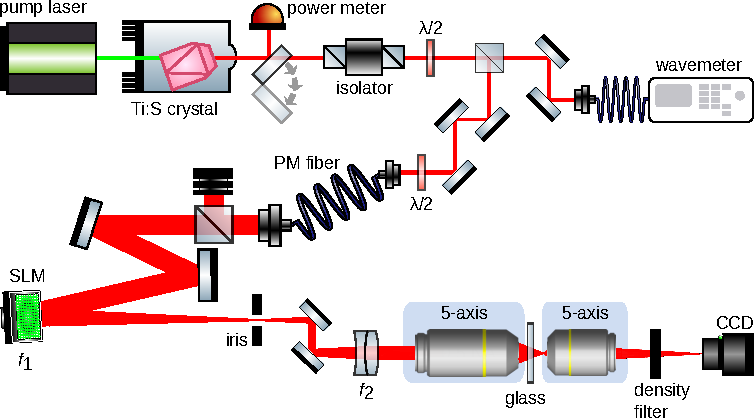
\includegraphics[width=0.95\linewidth]{figures/TiSandSLM.pdf}
    \caption{Output from a titanium sapphire ring laser is coupled into a polarization-maintaining fiber bringing it to the main table. 
    After alignment of the polarization direction, a spatial light modulator $f_1$ and achromatic lens $f_2 = 300$ mm feed the light into the Mitutoyo 0.5 NA objective.
    A glass plate serves to replace the vacuum viewport.
    The tweezer potential is imaged on a camera using a 0.85 NA microscope objective.
    The cubes shown are polarizing.}
    \label{fig:TiSandSLMsetup}
\end{figure}

\subsection{Calibration Imaging System}\label{subsec:CameraCalibration}

The 60X magnification of the 0.85 NA objective is only specified when used in a microscope with standard tube length distance, because it is finite conjugate corrected.
Outside of a standard microscope, we have to calibrate its exact magnification.
We do this using a high resolution target\footnote{Technologie Manufaktur TC-RT01}, featuring groups of lines with variable spacing between them. 
The way this was done is shown in \cref{fig:SetupResolutionTarget}.
Initially, we tried to use laser light to illuminate the target, but we did not get a clear image. 
Most likely this is because of the diffracting beams interfering with each other. 
To combat this we used light from an incoherent light source (\ac{LED}). 
We neglect the slightly different focus point from the Newport objective for our laser frequency compared to white light. 
An image of the calibration target showing the spaced lines is shown in \cref{fig:resolutionTarget}.

\begin{figure}
	\begin{subfigure}{.5\textwidth}
	    \flushleft
	    
\includegraphics[height=1.44cm]{figures/white.jpeg}
	    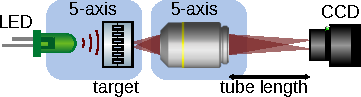
\includegraphics[width=\linewidth]{figures/LEDcalibration.pdf}
	    
\includegraphics[height=1.44cm]{figures/white.jpeg}
		\caption{}
		\label{fig:SetupResolutionTarget}
	\end{subfigure}
	\hfill
	\begin{subfigure}{.45\textwidth}
	    \flushright
		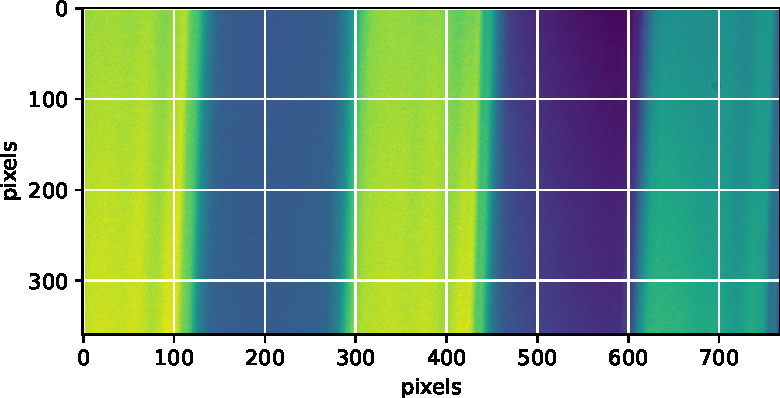
\includegraphics[width=\linewidth]{figures/LineSpacingCalibration.pdf}
		\caption{}
		\label{fig:3Dwaistfit}
	\end{subfigure}
	\caption{\textbf{a)} Illumination of the calibration target by an LED, imaged by the 0.85 NA objective and camera at fixed distance.
	\textbf{ b)} Image from the resolution target illuminated showing lines spaced by 45 lines per mm.}
	\label{fig:resolutionTarget}
\end{figure}

To detect the edges in \cref{fig:resolutionTarget}, we use an edge detection algorithm script.
For several 1D row slices of the image, it blurs the edge using a Gaussian to suppress noise and subsequently computes the spatial derivative. 
When the derivative surpasses a set threshold we define it as an edge.
Dividing the pixel spacing of the lines by the pixel pitch of the camera ($4.65$ $\mu$m) we find a magnification of ($67 \pm 3$)X, which is larger than the 60X specified by Newport. 
We attribute this to a slightly longer objective-camera distance that was used. 
After the calibration was performed the calibration target was removed and the setup in \cref{fig:TiSandSLMsetup} was used again, the objective-camera distance was kept constant for the remainder of the measurements.

\section{Results: Radial Dependency}\label{sec:TweezerRadial}

An image of the tweezer at the point of maximum intensity imaged onto a camera through the 0.85 NA objective is shown in fig. \ref{fig:2Dresults}a. 
The Airy ring is somewhat asymmetric, suggesting a slight tilt aberration is present.
This slight tilt is difficult to eliminate, as the alignment of the beam with the two objectives, glass plate and camera cannot be independently adjusted: tilting the first objective for example, will change the alignment of the incoming beam as well as the alignment with the glass plate and second objective.
Thus, the aberration could be a result of the imaging onto the camera and not from the potential itself.
In \cref{fig:2Dresults}, an aberration correction using the \ac{SLM} was already applied, but this turned out to have little effect on the radial intensity distribution.
This correction did have a significant effect on the axial (longitudinal) distribution however, therefore it will be explained in the next section (\cref{sec:Tweezer3D}).

Going back to fig. \ref{fig:2Dresults}a, we computed an azimuthal average of the radial intensity distribution which is shown in fig. \ref{fig:2Dresults}b.
This was done by integrating the amount of pixel counts in 'rings' around the center pixel.
The rings have a width of 1 pixel, such that the intensity as a function of the distance to the center in pixels can be computed using this binning method.
Next, pixel values are converted to microns using the calibration described in \cref{subsec:CameraCalibration}.
The measurement is compared against the Airy function or the ideal \ac{PSF} of the objective \cref{eq:NormalizedPSF} when using a uniform input beam, as well as the result from scalar diffraction theory using a Gaussian input beam equal to the aperture $w_i \sim R$, which was used to obtain the measurements.
The latter theoretical result was obtained by integrating \cref{eq:FourierBesselAperture} as a function of the radial coordinate $r$.
From \ref{fig:2Dresults}b, the Gaussian input beam results in a slightly ($\sim 9\%$) broader spot.
Additionally, the rings of the Airy disk will be slightly suppressed, this effect is known as Gaussian apodization.
This apodization effect is not that clearly visible in the measurements, but again this could be a result of an aberration.
Comparing the measurement to the theory result, the measurement has a waist which is about $\sim 10\%$ broader. Possibly, this is a result of convolution of the tweezer with the \ac{PSF} of the imaging system. Though the second objective has a significantly higher NA, the convolution effect can have significant contribution.

\begin{figure}
    \centering
    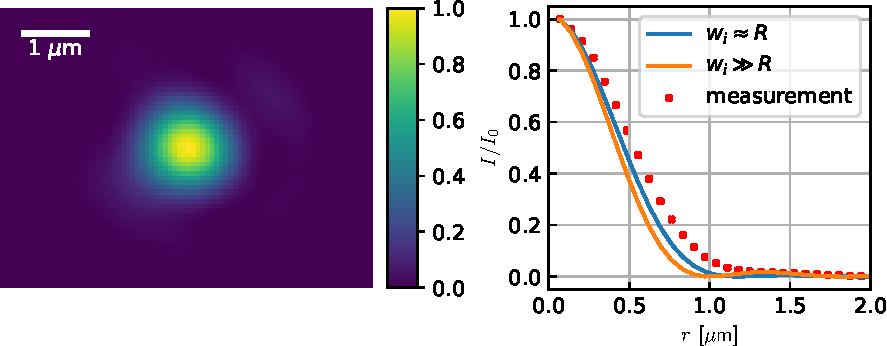
\includegraphics[width=\linewidth]{figures/AzimuthalAverageSpotZoomed.pdf}
    \caption{\textbf{a)} Tweezer as imaged by the second objective onto the CCD camera. 
	\textbf{ b)} Azimuthal average (red) plotted against the ideal \ac{PSF}, \cref{eq:NormalizedPSF} of the objective as well as the result from diffraction theory \cref{eq:FourierBesselAperture} for the input waist used.}
    \label{fig:2Dresults}
\end{figure}

To check if this is indeed the case, a more accurate analysis method is needed.
For example: in the previous binning method, the exact center location is not determined: it could lie anywhere in the center pixel. 
Also, information is lost during the binning. 
Therefore we also perform a two-dimensional fit using a normalized Gaussian $G/G_0$ in Cartesian coordinates (eq. \ref{eq:GaussianBeamIntensity})

\begin{equation}\label{eq:2DGaussian}
    \frac{G(x,y)}{G_0} =  
    \exp{\left[ -\frac{(x-x_0)^2}{2\sigma_x^2}\right]}
    \exp{\left[ -\frac{(y-x_0)^2}{2\sigma_y^2}\right]}.
\end{equation}
The result of this fit is shown in \cref{fig:3Dshowing}. 
Clearly, the obtained tweezer potential fits very well to a Gaussian, which justifies the assumption of using a Gaussian approximation to estimate the trap frequencies (\cref{eq:GaussianPotential}. 
This is confirmed by the coefficient of determination $R^2 > 0.99$.

\begin{figure}
\centering
	\begin{subfigure}{.49\textwidth}
	    \centering
		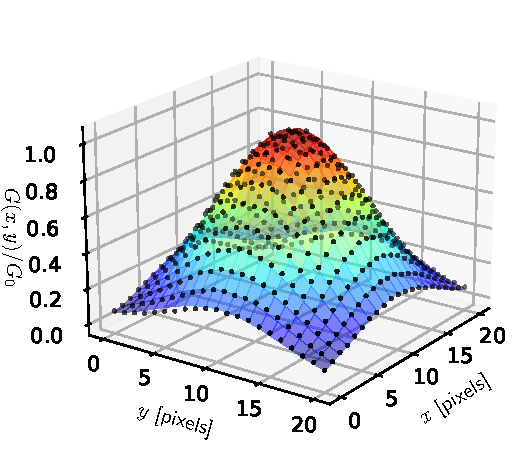
\includegraphics[width=0.96\linewidth]{figures/3DSpotFitGaussian.pdf}
		\caption{}
		\label{fig:3Dshowing}
	\end{subfigure}
	\begin{subfigure}{.49\textwidth}
		\centering
		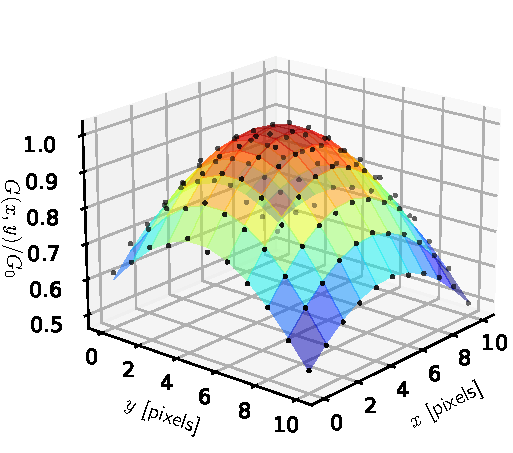
\includegraphics[width=0.96\linewidth]{figures/3DSpotFitGaussianSmaller.pdf}
		\caption{}
		\label{fig:3Dwaistfit}
	\end{subfigure}
	\caption{\textbf{a)} Plot showing convergence of the Gaussian fit.
	\textbf{b)} Region of interest around the maximum that was used to extract the waist. For both plots: $R^2>0.99$, but it is higher for the fit in \textbf{b}.}
	\label{fig:3Dfits}
\end{figure}

In order to extract the waist from \cref{fig:3Dshowing}, only the center $10 \times 10$ pixel area was considered as the Gaussian approximation works best for small $r$. 
And indeed the fit for smaller region of interest has had even higher $R^2$.
The result of this fit is shown in \cref{fig:3Dwaistfit}.
Assuming the $\sigma_x \sim \sigma_y$ which should be valid for a circular aperture, we find the waist as $w_{\text{image}} = 2\sigma = \sigma_x + \sigma_y = (0.88 \pm 0.04)$ $\mu$m, where the error originates mainly from the calibration of the magnification. 
Despite the 0.85 NA used, there will still be a slight convolution with the imaging point spread function present. 
Although in deconvolution is non-trivial in general, for the specific case of a Gaussian function, the deconvolved waist $w_{\text{object}}$ can be found in terms of the waists of the image $w_{\text{image}}$ and the diffraction-limited waist of the imaging system $w_{\text{system}}$ according to \cite{Knottnerus2018}

\begin{equation}\label{eq:Deconvolution}
    w_{\text{object}} = \sqrt{w_{\text{image}}^2-w_{\text{system}}^2}.
\end{equation}
This yields $w_{\text{object}} = (0.77 \pm 0.05)$ $\mu$m. 
Comparing to the theory result, for $\lambdaup = 820$ nm and $\text{NA} = 0.5$ (\cref{eq:Abbe,eq:GaussianAiryFit}) yields $w_0 = 0.689$ $\mu$m. 
But this result not possible because of using input beam size $w_i \sim R$. 
We know that as a result of this, the waist should be $\approx$9-10\% larger \cite{Sortais2007,Chon2007} which was confirmed by \cref{eq:FourierBesselAperture}, yielding $w_0 \sim 0.75$ $\mu$m, which is in good agreement with the result from diffraction theory.
We conclude the spot size of the tweezer is nearly diffraction-limited.

\section{Results: Axial Dependency}\label{sec:Tweezer3D}

To obtain tweezers with the smallest possible volume in order to load single atoms, not only the radial dependency on the intensity distribution is important, but the axial distribution as well.
The relevant parameter here is the Rayleigh range (see \cref{fig:GaussianBeam}).
To study the axial direction, we scan the Mitutoyo objective along the optical axis $z$ using a motorized stage and record an image of the radial profile of the tweezer for each step.
The relevant part of the optical setup for this is shown in \cref{fig:ZScanSetup}.
In the end, all images are stitched together to make a single image that would give an idea of a side view of the tweezer.

\begin{figure}
    \centering
    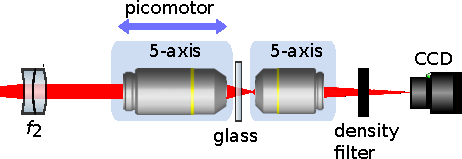
\includegraphics[width=0.6\linewidth]{figures/ZScanSetup.pdf}
    \caption{Optical setup for determining the axial dimension of the tweezer potential. The first objective was scanned along the optical axis using a piezo linear translation stage.}
    \label{fig:ZScanSetup}
\end{figure}


\subsection{Piezo Stage Calibration}

Piezo attenuated stages are very good at producing minuscule ($<30$ mm) step sizes in a repeatable fashion.
The stage we used is 8081-M 5-axis motorized tilt aligner from Newport. 
Because of the 5 degrees of freedom, it can accurately align the two objectives with each other. 
To drive this stage, we used a set of Newport 8742 controllers in daisy-chain configuration: both can drive 4 motors so we have 2 of them to address all 5 motors.
For scanning the axial direction of the tweezer we only use one of the 5 motors in the stage. 
However, to know the exact step size calibration is needed because the step size is dependent on the torque applied and the direction of travel.
In order to do this, we repeatedly measured the available translation range of some $\sim$ 3mm, recording the amount of steps this takes as well as the amount moved using a caliper. 
We found a step calibration of $10.6 \pm 0.3$ $\mu$m/step.

\subsection{Results}

In \cref{fig:AxialUncorrected} the scanned profile of the tweezer is shown prior to aberration correction using the \ac{SLM} is shown, as well as the maximum intensity recorded for each tweezer image normalized to the maximum intensity $I_0$ at the center of the tweezer.
Also plotted is the result from diffraction theory.
Clearly, there is a discrepancy between the two. 
We attributed this to the incorrect glass thickness used: the glass cell and corresponding glass plate consists of 4.0 mm thick quartz glass ($n=1.44$), whereas the cover glass correction of the objective was originally designed for 3.5 mm of N-BK7 glass ($n=1.51$).
The optical thickness $nd$ is thus 0.5 mm too large. 

\begin{figure}
\centering
	\begin{subfigure}{.49\textwidth}
	    \centering
		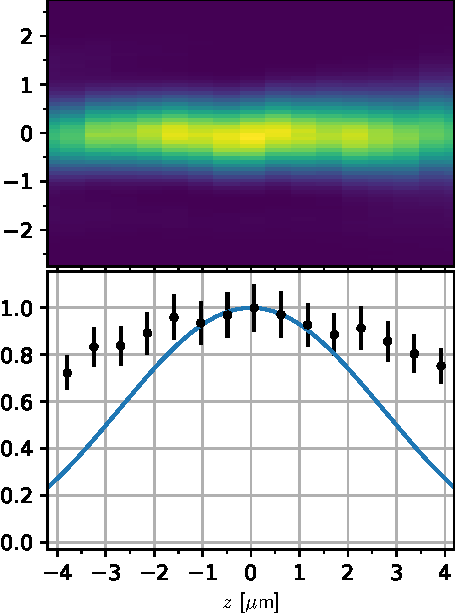
\includegraphics[height=9.5cm]{figures/AxialImageTweezerScanUncorrected.pdf}
		\caption{}
		\label{fig:AxialUncorrected}
	\end{subfigure}
	\begin{subfigure}{.49\textwidth}
		\centering
		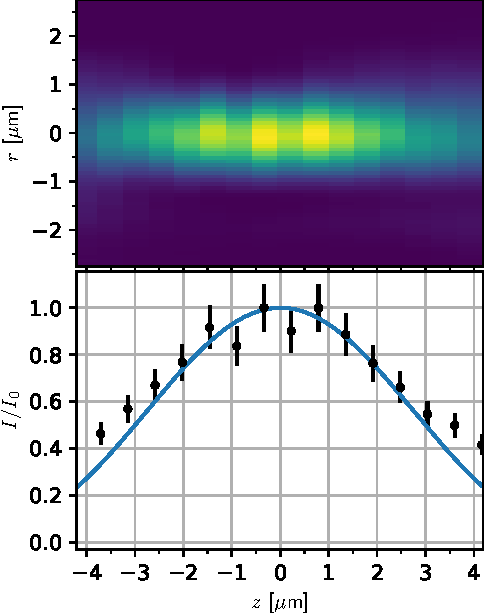
\includegraphics[height=9.5cm]{figures/AxialImageTweezerScan.pdf}
		\caption{}
		\label{fig:AxialZernike}
	\end{subfigure}
	\caption{Radial intensity profile \textbf{a)} before aberration correction: $z_R \sim 6.2$ $\mu$m and \textbf{b)} after aberration correction: $z_R \sim 3.5$ $\mu$m.}
	\label{fig:AxialScans}
\end{figure}

We can look at the effect of this material using the sketch in \cref{fig:SphericalSketch}. The extra glass has a thickness $d$ and refractive index $n$. 
To simplify calculations, the extra material is inserted on the right, but it can be positioned anywhere without effect on the change in focus $\delta z$ and in focus point location $\delta f$. The maximum ray angle is $\sin{\alpha_0} = R/f$. The refractive index of air is $n_0$ which will be assumed to be unity.
Now, the change of focus point is derived to be \cite{Iwaniuk2011}

\begin{figure}
    \centering
    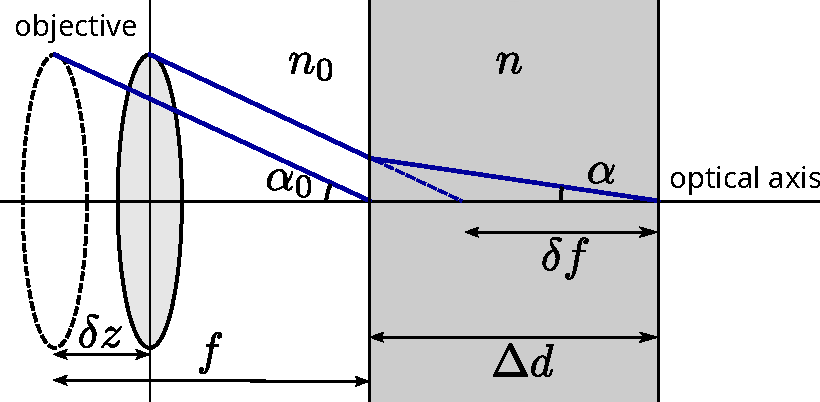
\includegraphics[width=0.65\linewidth]{figures/sphericalAberration.pdf}
    \caption{As a result of extra glass thickness $nd$, the objective will have to move a distance $\delta z$, corresponding to a change in focus distance $\delta f$.
    Figure adapted from from \cite{Iwaniuk2011}.}
    \label{fig:SphericalSketch}
\end{figure}


\begin{equation}\label{eq:SphericalFocus}
    \delta f = d - \delta z = d \left[
    1 - \frac{n_r}{\sqrt{1+\tan^2{(\alpha_0)}\cdot(1-n_r^2)}}
    \right],
\end{equation}
where $n_r=n_0/n=1/n$ is the ratio of refractive indices and $\tan{\alpha_0} = r/f$ is the incident angle. 
So \cref{eq:SphericalFocus} is a function of $r$ and will not be the same for paraxial rays compared to rays having a larger incident angle (marginal rays). 
For paraxial rays, ($\alpha_0 \rightarrow 0$), \cref{eq:SphericalFocus} reduces to $d(1-n_r)$. 
Subtracting this from \cref{eq:SphericalFocus} and Taylor expanding up to fourth order in $\alpha_0$ yields 

\begin{equation}\label{eq:FocusDifference}
    \delta f_{\text{marginal}} - \delta f_{\text{paraxial}} \approx
    \frac{d \tan^2{\alpha_0}}{2n} (1-n_r^2) - \frac{3d \tan^4{\alpha_0}}{8n}(1-n_r^2)^2+\mathcal{O}(\tan\alpha_0^6).
\end{equation}
Multiplying \cref{eq:FocusDifference} with $2\pi(n-n_0)/\lambdaup$ and converting to a radial dependence as $\tan{\alpha_0}= \text{NA} \times r/R$ yields \cite{Iwaniuk2011}

\begin{equation}\label{eq:ConversionRadial}
    \phi(r) \approx \frac{\pi d}{\lambdaup}(1-n_r)\left[
    \left(\text{NA}\frac{r}{R}\right)^2(1-n_r^2)-\frac{3}{4}\left(\text{NA}\frac{r}{ R}\right)^4(1-n_r^2)^2
    \right].
\end{equation}
This is a function that can be decomposed in Zernike polynomials.
The Zernike polynomials are a set of orthogonal polynomials on the unit disk, related to optical aberrations. 
They allow for weighted decomposition of a wavefront function $\phi$ using weights $a_j$ and polynomials $Z_j$ according to

\begin{equation}\label{eq:Zernike}
    \phi(\rho,\theta) = \sum_{j=1}^\infty a_j Z_j(\rho,\theta)
\end{equation}
The terms $Z_j(\rho,\theta)$ can be written in terms of the radial Zernike functions $R_n^m(\rho)$ where $\rho=r/R$ is the normalized radial coordinate and double indices $m,n$ are obtained from $j$ as 

\begin{equation}\label{eq:ZernikeRadial}
    j = \frac{n(n+2)+l}{2}, \quad
    R_{n}^{m}(\rho)=
    \sum_{s=0}^{(n-m) / 2}
    \frac{(-1)^{s}(n-s) !}{s !\left((n+m)/2-s\right) !\left((n-m)/2-s\right) !} \rho^{n-2 s}
\end{equation}
for $n-m$ is even, and 0 for $n-m$ odd. Furthermore $n \leq 0$, $|m| \leq n$. But it turns out \cref{eq:ConversionRadial} only has to nonzero $R_n^m$ terms: $R_2^2 = \rho^2$, which is a defocus aberration and $R_4^4 =\rho^4$ which is a third order spherical aberration. It is not needed to correct the defocus aberration with the SLM, leaving only the spherical aberration term. \cref{fig:AberrationTerm}

\begin{figure}
    \centering
    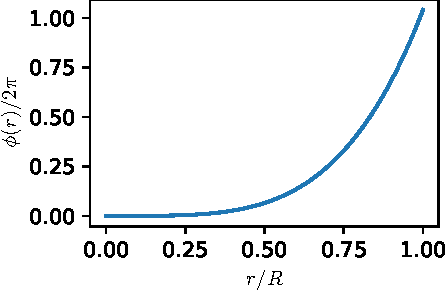
\includegraphics[width=0.4\textwidth]{figures/SphericalAberrationTerm.pdf}
    \caption{Phase correction applied onto the SLM to correct the third order spherical aberration as a function of the normalized radial coordinate $\rho=r/R$.}
    \label{fig:AberrationTerm}
\end{figure}


















